\documentclass[journal,12pt,twocolumn]{IEEEtran}

\usepackage{enumitem}
\usepackage{amsmath}
\usepackage{amssymb}
\usepackage{gensymb}
\usepackage{graphicx}
\usepackage{txfonts}         
\usepackage{listings}
\usepackage{lstautogobble}
\usepackage{mathtools}
\usepackage{bm}
\usepackage{hyperref}
\usepackage{polynom}
\usepackage{siunitx}
\usepackage{verbatim}
\usepackage[siunitx]{circuitikz}

\newcommand{\solution}{\noindent \textbf{Solution: }}
\providecommand{\pr}[1]{\ensuremath{\Pr\left(#1\right)}}
\providecommand{\brak}[1]{\ensuremath{\left(#1\right)}}
\providecommand{\cbrak}[1]{\ensuremath{\left\{#1\right\}}}
\providecommand{\sbrak}[1]{\ensuremath{\left[#1\right]}}
\providecommand{\mean}[1]{E\left[ #1 \right]}
\providecommand{\var}[1]{\mathrm{Var}\left[ #1 \right]}
\providecommand{\der}[1]{\mathrm{d} #1}
\providecommand{\gauss}[2]{\mathcal{N}\ensuremath{\left(#1,#2\right)}}
\providecommand{\mbf}{\mathbf}
\providecommand{\abs}[1]{\left\vert#1\right\vert}
\providecommand{\norm}[1]{\left\lVert#1\right\rVert}
\providecommand{\z}[1]{{\mathcal{Z}}\cbrak{#1}}
\providecommand{\ztrans}{\overset{\mathcal{Z}}{ \rightleftharpoons}}
\providecommand{\system}[1]{\overset{\mathcal{#1}}{ \longleftrightarrow}}
\providecommand{\parder}[2]{\frac{\partial}{\partial #2} \brak{#1}}

\let\StandardTheFigure\thefigure
\let\vec\mathbf

\numberwithin{equation}{section}
\numberwithin{figure}{section}
\renewcommand{\thefigure}{\theenumi}
\renewcommand\thesection{\arabic{section}}

\newcommand{\myvec}[1]{\ensuremath{\begin{pmatrix}#1\end{pmatrix}}}
\newcommand{\mymat}[1]{\ensuremath{\begin{bmatrix}#1\end{bmatrix}}}
\newcommand{\mydet}[1]{\ensuremath{\begin{vmatrix}#1\end{vmatrix}}}
\newcommand{\define}{\stackrel{\triangle}{=}}

\DeclareMathOperator*{\argmin}{arg\,min}
\DeclareMathOperator*{\argmax}{arg\,max}

\makeatletter
\def\pld@CF@loop#1+{%
    \ifx\relax#1\else
        \begingroup
          \pld@AccuSetX11%
          \def\pld@frac{{}{}}\let\pld@symbols\@empty\let\pld@vars\@empty
          \pld@false
          #1%
          \let\pld@temp\@empty
          \pld@AccuIfOne{}{\pld@AccuGet\pld@temp
                            \edef\pld@temp{\noexpand\pld@R\pld@temp}}%
           \pld@if \pld@Extend\pld@temp{\expandafter\pld@F\pld@frac}\fi
           \expandafter\pld@CF@loop@\pld@symbols\relax\@empty
           \expandafter\pld@CF@loop@\pld@vars\relax\@empty
           \ifx\@empty\pld@temp
               \def\pld@temp{\pld@R11}%
           \fi
          \global\let\@gtempa\pld@temp
        \endgroup
        \ifx\@empty\@gtempa\else
            \pld@ExtendPoly\pld@tempoly\@gtempa
        \fi
        \expandafter\pld@CF@loop
    \fi}
\def\pld@CMAddToTempoly{%
    \pld@AccuGet\pld@temp\edef\pld@temp{\noexpand\pld@R\pld@temp}%
    \pld@CondenseMonomials\pld@false\pld@symbols
    \ifx\pld@symbols\@empty \else
        \pld@ExtendPoly\pld@temp\pld@symbols
    \fi
    \ifx\pld@temp\@empty \else
        \pld@if
            \expandafter\pld@IfSum\expandafter{\pld@temp}%
                {\expandafter\def\expandafter\pld@temp\expandafter
                    {\expandafter\pld@F\expandafter{\pld@temp}{}}}%
                {}%
        \fi
        \pld@ExtendPoly\pld@tempoly\pld@temp
        \pld@Extend\pld@tempoly{\pld@monom}%
    \fi}
\makeatother

\lstset {
	frame=single, 
	breaklines=true,
	columns=fullflexible,
	autogobble=true
}             

\begin{document}


	\section{Bilinear Transform}
	\begin{enumerate}[label=\thesection.\arabic*.,ref=\thesection.\theenumi]
	\item In Fig. \ref{fig:ckt}, consider the case when $S$ is switched to $Q$ right in the beginning. Formulate the differential equation
	
	\solution The differential equation is the same as before 
	\begin{align}
		&\frac{v_c(t) - 0}{R_1} + \frac{v_c(t) - v_2(t)}{R_2} + \frac{\der{q}}{\der{t}} = 0 \\
		\text{i.e., } &\frac{v_c(t)}{R_1} + \frac{v_c(t) - v_2(t)}{R_2} + C_0\frac{\der{v_c}}{\der{t}} = 0
	\end{align}
	
	but with a different initial condition
	\begin{equation}
		q(0^-) = q(0) = 0
	\end{equation}
	
	\item Find $H(s)$ considering the ouput voltage at the capacitor
	
	\solution On taking the Laplace transform on both sides of this equation
	\begin{align}
		&\frac{V_c(s)}{R_1} + \frac{V_c(s) - V_2(s)}{R_2} + sQ(s) - 0 = 0 \\
		\implies &V_c(s) \brak{\frac{1}{R_1} + \frac{1}{R_2}} + sC_0V_c(s) = \frac{V_2(s)}{R_2} \\
		\implies &\frac{V_c(s)}{V_2(s)} = \frac{\frac{1}{R_2}}{\frac{1}{R_1} + \frac{1}{R_2} + sC_0}
	\end{align}
	
	The transfer function is thus
	\begin{align}
		H(s) = \frac{\frac{1}{R_2C_0}}{s + \frac{1}{R_1C_0} + \frac{1}{R_2C_0}}
	\end{align}
	
	On substituting the values, we get
	\begin{equation}
		H(s) = \frac{5 \times 10^5}{s + 1.5 \times 10^6}
	\end{equation}
	
	\item Plot $H(s)$.  What kind of filter is it?
	
	\solution Download the following Python code that plots Fig. \ref{fig-4.3}
	\begin{lstlisting}
		wget https://github.com/Ankit-Saha-2003/EE3900/raw/main/Circuit/codes/4.3.py
	\end{lstlisting}
	
	Run the codes by executing
	\begin{lstlisting}
		python 4.3.py
	\end{lstlisting}	
	
	\begin{figure}[!ht]
		\centering
		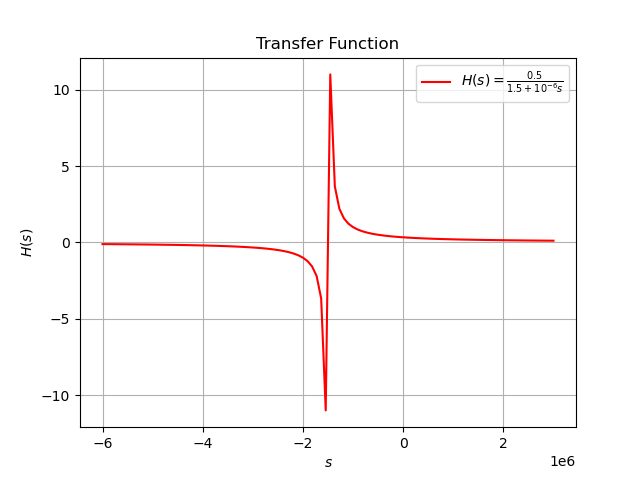
\includegraphics[width=\columnwidth]{./figs/4.3.png}
		\caption{Plot of $H(s)$}
		\label{fig-4.3}	
	\end{figure}
	
	Consider the frequency-domain transfer function by putting $s = \j\omega$
	\begin{align}
		H(\j\omega) &= \frac{5 \times 10^5}{\j\omega + 1.5 \times 10^6} \\
		\implies \abs{H(\j\omega)} &= \frac{5 \times 10^5}{\sqrt{\omega^2 + 2.25\times10^{12}}}
	\end{align}
	
	As $\omega$ increases, $\abs{H(\j\omega)}$ decreases
	
	In other words, the amplitude of high-frequency signals gets diminished and they get filtered out
	
	Therefore, this is a low-pass filter
	
	\item Using trapezoidal rule for integration, formulate the difference equation by considering 
	\begin{align}
		y(n) = y(t)\vert_{t=n}
	\end{align}
	
	\solution
	\begin{align}
		&\frac{v_c(t)}{R_1} + \frac{v_c(t) - v_2(t)}{R_2} + C_0\frac{\der{v_c}}{\der{t}} = 0 \\
		\implies &C_0\frac{\der{v_c}}{\der{t}} = \frac{2u(t)-v_c(t)}{R_2} - \frac{v_c(t)}{R_1} \\
		\implies &\left.v_c(t)\right|_{t=n}^{n+1} = \int_{n}^{n+1} \brak{\frac{2u(t)-v_c(t)}{R_2C_0} - \frac{v_c(t)}{R_1C_0}} \der{t}
	\end{align}
	
	By the trapezoidal rule of integration
	\begin{align}
		\int_a^b f(t) \der{t} \approx \frac{b-a}{2} (f(a) + f(b))
	\end{align}
	
	Consider $y(t) = v_c(t)$
	\begin{multline}
		y(n+1) - y(n) = \frac{1}{R_2C_0}\brak{u(n)+u(n+1)} \\
		- \frac12(y(n+1) + y(n))\brak{\frac{1}{R_1C_0} + \frac{1}{R_2C_0}}
	\end{multline}
	
	Thus, the difference equation is
	\begin{multline}
		y(n+1) \brak{1 + \frac{1}{2R_1C_0} + \frac{1}{2R_2C_0}} \\= y(n) \brak{1 - \frac{1}{2R_1C_0} - \frac{1}{2R_2C_0}} \\+ \frac{1}{R_2C_0}\brak{u(n)+u(n+1)}
	\end{multline}
	
	\item Find $H(z)$
	
	\solution Let $\z{y(n)} = Y(z)$
	
	On taking the $Z$-transform on both sides of the difference equation
	\begin{multline}
		zY(z)\brak{1 + \frac{1}{2R_1C_0} + \frac{1}{2R_2C_0}} \\= Y(z)\brak{1 - \frac{1}{2R_1C_0} - \frac{1}{2R_2C_0}} \\+ \frac{1}{R_2C_0} \brak{\frac{1}{1-z^{-1}} + \frac{z}{1-z^{-1}}}
	\end{multline}
	\begin{multline}
		Y(z)\brak{z + \frac{z}{2R_1C_0} + \frac{z}{2R_2C_0} - 1 + \frac{1}{2R_1C_0} + \frac{1}{2R_2C_0}} \\
		= \frac{1}{R_2C_0} \frac{1+z}{1-z^{-1}}
	\end{multline}
	
	Also
	\begin{align}
		v_2(t) &= 2 &&\forall t \ge 0\\
		\implies x(n) &= 2u(n) \\
		\implies X(z) &= \frac{2}{1-z^{-1}} &&\abs{z} > 1
	\end{align}
	
	Thus, the transfer function in $z$-domain is
	\begin{align}
		H(z) &= \frac{Y(z)}{X(z)} \\
		&= \frac{\frac{1+z}{2R_2C_0}}{z + \frac{z}{2R_1C_0} + \frac{z}{2R_2C_0} - 1 + \frac{1}{2R_1C_0} + \frac{1}{2R_2C_0}} \\
		&= \frac{\frac{1 + z^{-1}}{2R_2C_0}}{1 + \frac{1}{2R_1C_0} + \frac{1}{2R_2C_0} - z^{-1} + \frac{z^{-1}}{2R_1C_0} + \frac{z^{-1}}{2R_2C_0}}
	\end{align}
	
	On substituting the values
	\begin{align}
		H(z) &= \frac{2.5\times10^5 (1+z^{-1})}{7.5\times10^5 + 1 + (7.5\times10^5 - 1)z^{-1}}
	\end{align}
	
	with the ROC being
	\begin{align}
		\abs{z} &> \max\brak{1, \abs{\frac{7.5\times10^5 - 1}{7.5\times10^5 + 1}}} \\
		\implies \abs{z} &> 1
	\end{align}
	
	\item How can you obtain $H(z)$ from $H(s)$?
	
	\solution The $Z$-transform can be obtained from the Laplace transform by the substitution
	\begin{align}
		s &= \frac{2}{T} \frac{1-z^{-1}}{1+z^{-1}}
	\end{align}
	where $T$ is the step size of the trapezoidal rule ($1$ in our case)
	
	This is known as the bilinear transform
	
	Thus
	\begin{align}
		H(z) &= \frac{\frac{1}{R_2C_0}}{2\frac{1-z^{-1}}{1+z^{-1}} + \frac{1}{R_1C_0} + \frac{1}{R_2C_0}} \\
		&= \frac{\frac{1 + z^{-1}}{2R_2C_0}}{1-z^{-1}	 + \brak{\frac{1}{2R_1C_0} + \frac{1}{2R_2C_0}}(1 + z^{-1})} \\
		&= \frac{\frac{1 + z^{-1}}{2R_2C_0}}{1 + \frac{1}{2R_1C_0} + \frac{1}{2R_2C_0} - z^{-1} + \frac{z^{-1}}{2R_1C_0} + \frac{z^{-1}}{2R_2C_0}} \\
		&= \frac{2.5\times10^5 (1+z^{-1})}{7.5\times10^5 + 1 + (7.5\times10^5 - 1)z^{-1}}
	\end{align}
	which is the same as what we obtained earlier
	\end{enumerate}
	\end{document}